\begin{frame}{Robustness Result: COLORED OBJECTS/OBJECT COUNTING}
\small

\begin{columns}[T]
\begin{column}{0.52\linewidth}
\centering
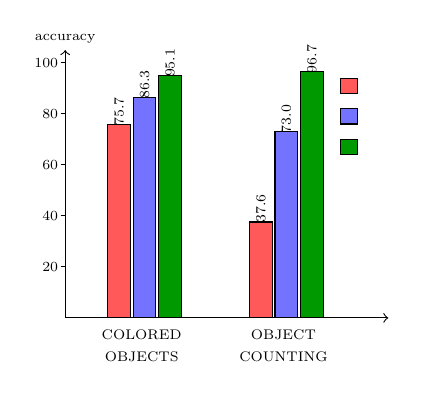
\begin{tikzpicture}[scale=0.72, transform shape, x=1cm, y=0.045cm]

% Axes
\draw[->] (0,0) -- (5.7,0) node[right]{};
\draw[->] (0,0) -- (0,105) node[above]{\scriptsize accuracy};

% Y ticks
\foreach \y in {20,40,60,80,100}
    \draw (-0.08,\y) -- (0,\y)
    node[left]{\scriptsize \y};

% X labels
\node[align=center] at (1.35,-11) {\scriptsize COLORED\\[-1pt]\scriptsize OBJECTS};
\node[align=center] at (3.85,-11) {\scriptsize OBJECT\\[-1pt]\scriptsize COUNTING};

% COLORED OBJECTS
\draw[fill=red!65]          (0.75,0) rectangle (1.15,75.7);
\draw[fill=blue!55]         (1.20,0) rectangle (1.60,86.3);
\draw[fill=green!60!black]  (1.65,0) rectangle (2.05,95.1);

% OBJECT COUNTING
\draw[fill=red!65]          (3.25,0) rectangle (3.65,37.6);
\draw[fill=blue!55]         (3.70,0) rectangle (4.10,73.0);
\draw[fill=green!60!black]  (4.15,0) rectangle (4.55,96.7);

% Value labels
\node[rotate=90] at (0.95,81.0) {\scriptsize 75.7};
\node[rotate=90] at (1.40,91.5) {\scriptsize 86.3};
\node[rotate=90] at (1.85,100.0) {\scriptsize 95.1};

\node[rotate=90] at (3.45,43.0) {\scriptsize 37.6};
\node[rotate=90] at (3.90,78.0) {\scriptsize 73.0};
\node[rotate=90] at (4.35,101.5) {\scriptsize 96.7};

% Legend
\draw[fill=red!65]         (4.85,88) rectangle (5.15,94);
\node[right] at (5.2,91) {\scriptsize \Direct{}};

\draw[fill=blue!55]        (4.85,76) rectangle (5.15,82);
\node[right] at (5.2,79) {\scriptsize \CoT{}};

\draw[fill=green!60!black] (4.85,64) rectangle (5.15,70);
\node[right] at (5.2,67) {\scriptsize \PAL{}};

\end{tikzpicture}\\
\source{PAL paper, Table 2 and Section 5.2.}
\begin{block}{Observation}
On both selected symbolic/algorithmic tasks, \PAL{} performs best.
\end{block}

\end{column}

\begin{column}{0.45\linewidth}


\begin{block}{Why PAL helps}
These tasks can be translated into explicit program operations:
dictionaries for object--color lookup, lists for ordering, and counting/filtering loops for object categories.
\end{block}

\begin{block}{Why the gain is smaller}
The tasks are less arithmetically fragile than GSM-HARD: \CoT{} can already solve many cases by tracking the objects in text, so \PAL{} mainly reduces bookkeeping errors rather than fixing difficult calculations.
\end{block}
\end{column}
\end{columns}


\end{frame}